%\thispagestyle{empty}
\section{FUNDAMENTAÇÃO TEÓRICA}

%\pagestyle{headings}
%\pagenumbering{arabic}

\subsection{EVERIS}
A Everis é uma multinacional, presente em dezesseis países, do ramo de consultoria e outsourcing. Há dois anos ela incorporou-se ao grupo NTT DATA, que é uma das dez maiores empresas de serviços na área de tecnologia da informação do mundo. Segundo informações contidas no site da empresa, mais de 19.000 profissionais espalhados pela América Latina, Europa e EUA compõem o quadro de funcionários da empresa.

\subsubsection{Serviços}
Os principais serviços oferecidos pela empresa são:

•	Consultoria: a Everis presta assessoria de qualidade aos seus clientes com o objetivo de aprimorar suas atividades e processos de gestão. Auxiliando-os a crescer de forma inteligente e sustentável.

•	Transformação digital: a Everis auxilia seus clientes a reinventar e aperfeiçoar seus processos e suas plataformas tecnológicas.

•	Tecnologia: a Everis seleciona, implementa e otimiza tecnologias e soluções empresariais para acelerar o processo da transformação digital. Ela identifica as necessidades e os desejos dos clientes para construir produtos digitais eficientes e sustentáveis.

\subsubsection{Áreas de atuação e clientes}
•	Bens de consumo – entre os serviços ofertados aos clientes desta área, pode-se destacar as soluções de televendas para a empresa Danone, uma multinacional de produtos alimentícios.

•	Serviço público – nesta área é possível destacar o serviço prestado ao governo espanhol, a digitalização do Registro Civil espanhol para o Ministério da Justiça.

•	Mídia e telecomunicações –  o maior cliente da Everis neste setor é a empresa Telefónica, uma multinacional espanhola de telecomunicações que engloba marcas como: Movistar (Espanha e Hispano América), O2 (Europa) e VIVO (Brasil).

\subsection{SELENIUM}
Segundo Selenium Hq (2017)\nocite{SELENIUMHQ}, o Selenium é um conjunto de ferramentas open source para automação de web browsers, ou seja, é principalmente utilizado para automação de testes em aplicações web. Ele possui suporte para os principais navegadores, tais como Firefox, Chrome, IE, Safari, entre outros. Ele é composto pelas seguintes ferramentas:

•	Selenium IDE: É um plugin do Firefox (a partir do Firefox 2) para o desenvolvimento de testes automatizados e que possibilita a gravação das ações que são executadas criando um script em formato HTML, que pode ser exportado para linguagens de programação, como Java, C\#, PHP, Python, Ruby, entre outras. 

•	Selenium Remote Control (RC): Também conhecido como Selenium 1, o Selenium RC era um sistema cliente/servidor utilizado para executar scripts em navegadores diferentes do Firefox, porém está ultrapassado, tendo sido substituído pelo Selenium WebDriver.

•	Selenium WebDriver: Também chamado de Selenium 2, o Selenium WebDriver é uma junção do Selenium 1 e do WebDriver, um projeto criado pela Google como forma de resolver as limitações do Selenium RC. Ele é um conjunto de bibliotecas, suportado pelas linguagens Java, Python, Ruby e C\#, utilizado para criação e alteração de scripts de teste. Ele automatiza as entradas de dados no navegador, realizando ações como clicks, submissão de formulários, inserção de dados em inputs, etc. Esta foi a ferramenta do Selenium utilizada durante o treinamento e o estágio.

A Figura \ref{selenium} apresenta um exemplo de automação do preenchimento de uma página Web. Após obter o Drive do Chrome (Classe WebDriver), é possível realizar operações no browser através de seus métodos navigate, findElement, sendKeys, etc.

\begin{figure}[htb]
  \begin{center}
    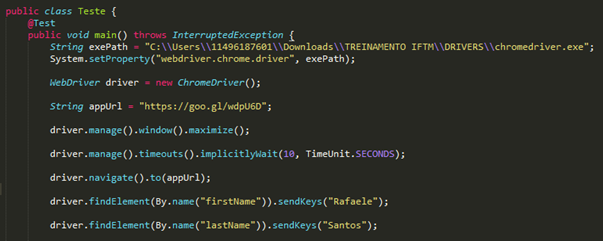
\includegraphics[scale=0.85]{Imagens/selenium.png}
  \end{center}
  \caption{Exemplo de utilização do Selenium Web Driver
Fonte: Elaborada pelo autor (2018)}
  \label{selenium}
\end{figure}

\textbf{\subsection{$E-FA^{3}$}}
O e-FA3 é uma ferramenta privada, desenvolvida pela Everis que permite a manipulação dos frameworks utilizados para a automação de teste, como Selenium WebDriver, que tem como objetivos facilitar a integração dos testes com a massa de dados de entrada que são recebidos em forma de planilha e simplificar a emissão de evidências (screenshots) da execução do teste e a comparação do resultado final.

\subsection{JUNIT}
É um framework open source, criado pelo cientista da computação Erich Gamma e pelo engenheiro de software Kent Beck, utilizado para criação e manutenção de unidades de teste de código Java, que verifica se o resultado gerado pelo método é o esperado, ou seja, ele compara esses resultados e informa se os testes foram executados corretamente ou se falharam. \nocite{Dias2014}

\subsection{EXCEL}
Excel é um editor de planilhas desenvolvido pela empresa Microsoft, amplamente usado para a realização de operações financeiras e contabilísticas usando planilhas.
No e-FA3 a massa de dados do teste é recebida através de uma planilha. Durante estágio, o Excel foi utilizado para a parametrização da massa de dados (Figura \ref{excel}), ou seja, todos os dados de entrada importantes eram colocados na planilha, assim, caso houvesse alguma modificação na massa de dados, seria necessário alterar apenas na planilha e não no script. Na planilha também era colocado o resultado esperado de cada caso de teste para a comparação com o resultado obtido após a execução.

\begin{figure}[htb]
  \begin{center}
    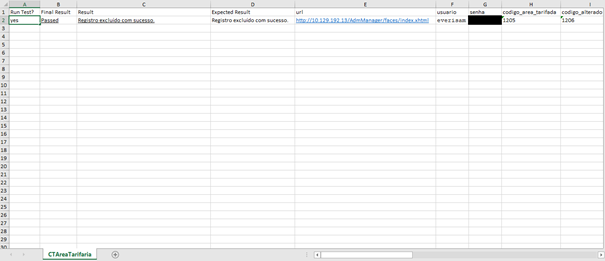
\includegraphics[scale=0.85]{Imagens/excel.png}
  \end{center}
  \caption{Figura 2 - Exemplo do uso do Excel para parametrização de dados
Fonte: Elaborada pelo autor (2018)}
  \label{excel}
\end{figure}

\subsection{LINGUAGEM JAVA}
A linguagem Java foi utilizada durante a criação dos scripts de testes. De acordo com Silveira (2003) \nocite{Silveira2003}, Java é uma linguagem orientada a objeto que foi criada pela empresa Sun Microsystems com o intuito inicial de ser utilizada em aparelhos eletrodomésticos e que solucionassem as falhas de outras linguagens da época. Sua principal característica é a portabilidade, permitindo que um código compilado possa ser executado em diversos ambientes diferentes.

\subsection{ECLIPSE IDE}
O Eclipse é uma IDE para de desenvolvimento de diversas linguagens, através do uso de plug-ins. Foi a IDE utilizada durante o estágio para o desenvolvimento na linguagem Java.